%----------------------------------------------------------------------------------------
%	PACKAGES AND OTHER DOCUMENT CONFIGURATIONS
%----------------------------------------------------------------------------------------

\documentclass[paper=a4, fontsize=11pt]{scrartcl} % A4 paper and 11pt font size
\usepackage{multicol}
\usepackage[T1]{fontenc} % Use 8-bit encoding that has 256 glyphs
\usepackage{fourier} % Use the Adobe Utopia font for the document - comment this line to return to the LaTeX default
\usepackage[english]{babel} % English language/hyphenation
\usepackage{amsmath,amsfonts,amsthm} % Math packages
\usepackage{listings}
\usepackage{lipsum} % Used for inserting dummy 'Lorem ipsum' text into the template
\usepackage{graphicx}
\usepackage{subfig}
\usepackage{float}

\usepackage{sectsty} % Allows customizing section commands
\allsectionsfont{\centering \normalfont\scshape} % Make all sections centered, the default font and small caps

\usepackage{fancyhdr} % Custom headers and footers
\pagestyle{fancyplain} % Makes all pages in the document conform to the custom headers and footers
\fancyhead{} % No page header - if you want one, create it in the same way as the footers below
\fancyfoot[L]{} % Empty left footer
\fancyfoot[C]{} % Empty center footer
\fancyfoot[R]{\thepage} % Page numbering for right footer
\renewcommand{\headrulewidth}{0pt} % Remove header underlines
\renewcommand{\footrulewidth}{0pt} % Remove footer underlines
\setlength{\headheight}{13.6pt} % Customize the height of the header

%\numberwithin{equation}{section} % Number equations within sections (i.e. 1.1, 1.2, 2.1, 2.2 instead of 1, 2, 3, 4)
%\numberwithin{figure}{section} % Number figures within sections (i.e. 1.1, 1.2, 2.1, 2.2 instead of 1, 2, 3, 4)
%\numberwithin{table}{section} % Number tables within sections (i.e. 1.1, 1.2, 2.1, 2.2 instead of 1, 2, 3, 4)

%\setlength\parindent{0pt} % Removes all indentation from paragraphs - comment this line for an assignment with lots of text

%----------------------------------------------------------------------------------------
%	TITLE SECTION
%----------------------------------------------------------------------------------------

\newcommand{\horrule}[1]{\rule{\linewidth}{#1}} % Create horizontal rule command with 1 argument of height

\title{	
\normalfont \normalsize 
\textsc{Syddansk Universitet} \\ [25pt] 
\horrule{0.5pt} \\[0.4cm] % Thin top horizontal rule
\huge Random Forests and Decision Trees \\ % The assignment title
\horrule{2pt} \\[0.5cm] % Thick bottom horizontal rule
}

\author{Bjarki Sigurdsson \\ Abdulrahman Abdulrahim \\ Miguel de la Colina \\ Group 5}
 % Your name

\date{\normalsize\today} % Today's date or a custom date

\begin{document}

\maketitle % Print the title

%----------------------------------------------------------------------------------------
%	PROBLEM 1
%----------------------------------------------------------------------------------------


\section*{Abstract}

\paragraph{The purpose of the exercise was to get familiar with random forests and decision trees and manage to get a grasp of how they work and how they function when using real data-sets in this case the ciphers.}
%The purpose of this report is to use the k-nearest neighbor algorithm on a data-set made of ciphers. We will be dividing the data into two sets, one for training and one for testing. We will analyze the results for different values of k and DPI to see how this alters our results. Also we will be applying the  Gaussian smoothing with various sigmas in order to see how does this alter the results.}  

%------------------------------------------------


%----------------------------------------------------------------------------------------
%	PROBLEM 2
%----------------------------------------------------------------------------------------

\section{Decision Trees}
In this section we will be working exclusively with decision trees finding optimal decision point, computing and visualizing one and also doing cross validation with the results that we manage to obtain. 

\subsection{Optimal decision point}
When using decision trees for classification with continuous variables, the common method involves, for each attribute, a threshold which maximizes information gain. Thresholding is a binary operation and thus does not generalize simply to multiclass problems such as this, but one workaround is to train multiple classifiers. Each of these is trained to classify a single class in a one vs. all manner. In computing the following results, we create a classifier for the 1 digit by computing the optimal decision point for each of the first five principal components. The method used for computing the threshold is simple: We sort on the current PC and iterate through the samples, testing each value as a threshold and computing the corresponding information gain.\par
 Figure \ref{fig:threshold} shows information gain as a function of data matrix row number for each of the five PCs. The thresholds chosen were the maxima of these graphs, 0.1136, 0.0463, 0.0298, 0.0457 and 0.0726 for components 1-5, respectively. Note that some of these gains are greater than those for preceding PCs. This shows the influence of specific PCs on the classification of the 1 digit and varies for other classes.
 \begin{figure}[h]
	\centering
	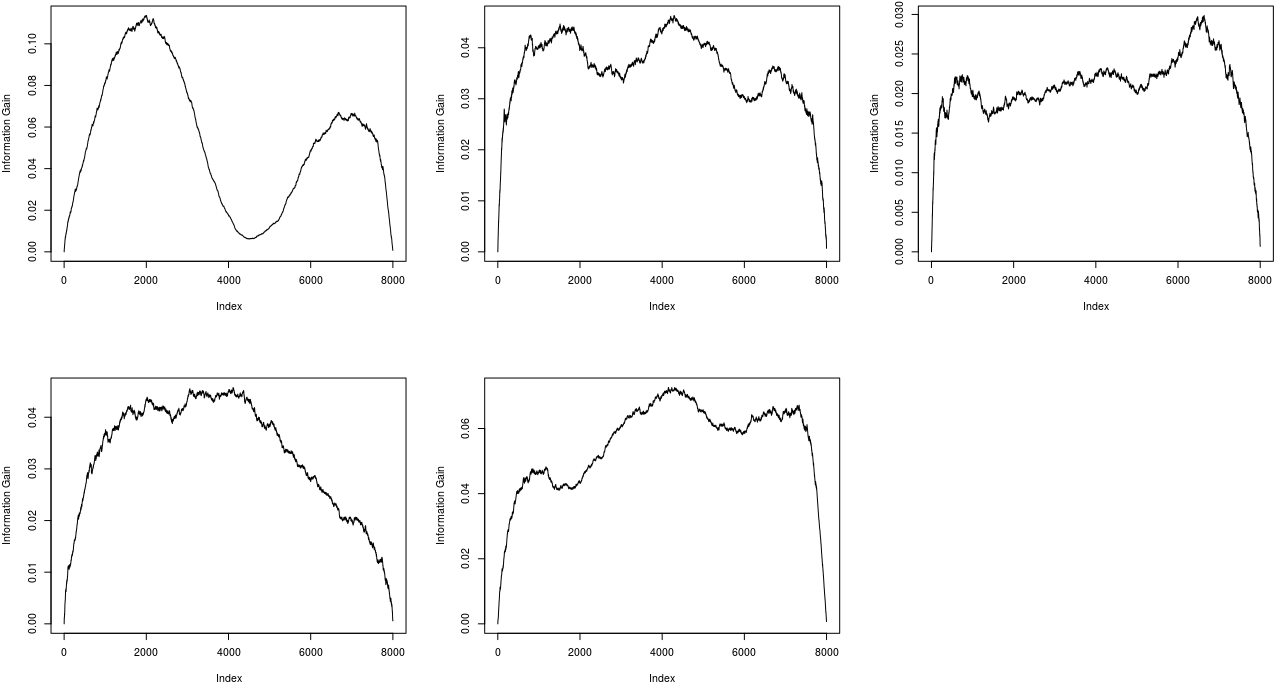
\includegraphics[width=0.8\textwidth]{figures/threshold.png}
	\caption{Decision Tree of person dependent set.}
	\label{fig:threshold}
\end{figure}

\subsection{Compute Decision Tree}

\begin{figure}[h]
	\centering
	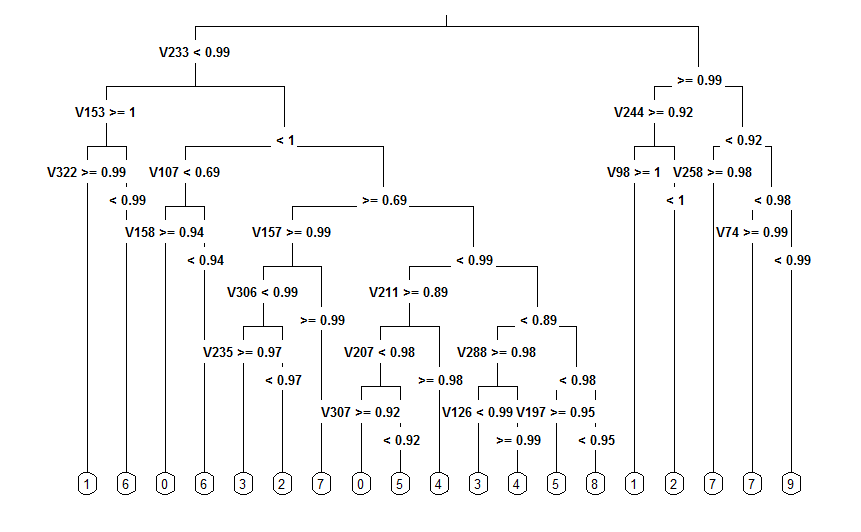
\includegraphics[width=0.8\textwidth]{figures/decisionTree.png}
	\caption{Decision Tree of person dependent set.}
	\label{fig:scree}
\end{figure}

\begin{figure}[h]
	\centering
	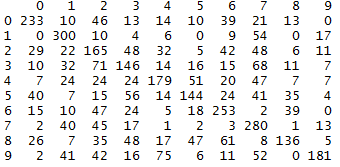
\includegraphics[width=0.8\textwidth]{figures/confusionMatrix.PNG}
	\caption{Confusion matrix of test set results and actual classes.}
	\label{fig:scree}
\end{figure}


In the second part of the exercise we used the person dependent data-set and split it into training and test sets and using rpart in r we created a model for a decision tree and as we can see in figure 1 that is the outcome that came from the actual decision tree once we tested the test set we actually got an accuracy of .5042 and as we can see from the confusion matrix in figure 2 the diagonal is where most of the results are showing that it had pretty reasonable result accuracy.


\clearpage
\subsection{Cross-Validation}
Now we made cross validation for the dependent set using 10\% as test set and the other 90\% as training and we can see on figure 3 that most of the results are around .53 showing a very consistent trend no matter which test and training sets we are using

\begin{figure}[h]
	\centering
	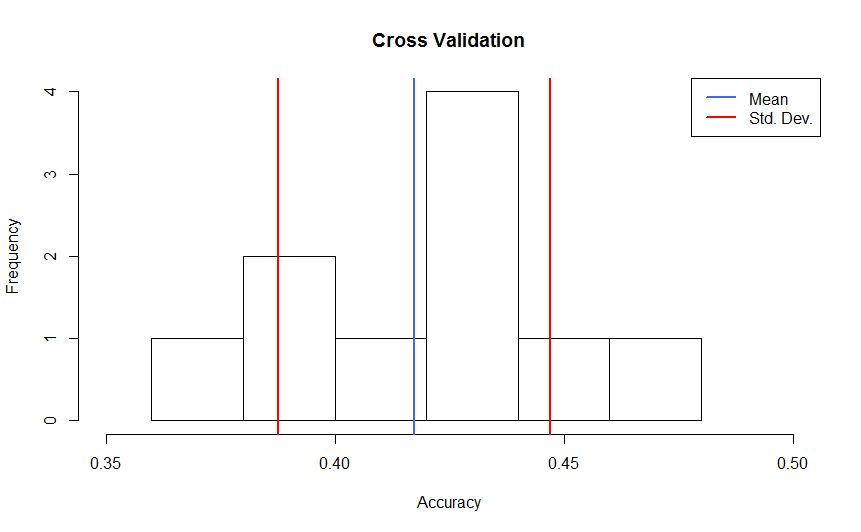
\includegraphics[width=0.8\textwidth]{figures/crossValidation.png}
	\caption{Decision Tree of person dependent set.}
	\label{fig:scree}
\end{figure}


\clearpage
\section{Random Forests}
Random forests are robust classifiers which use the majority vote of multiple decision trees for classification. This method uses bootstrap aggregation to circumvent the overfitting inherent to decision trees.\par
There are two main parameters to tune when constructing a decision tree, namely the total number of trees and their depth. A higher total number of trees tends to reduce overall classification error with diminishing results. In other words, adding trees reduces the error but the error will eventually converge. The tree depth contributes to the classifier's level of overfitting. Deeper trees tend to overfit data so if the data is noisy, then pruning is recommended and often implemented by simply limiting the tree depth. 

\end{document}
\grid
